\documentclass[9pt,a4paper,]{extarticle}

\usepackage{f1000_styles}

\usepackage[pdfborder={0 0 0}]{hyperref}

\usepackage[numbers]{natbib}
\bibliographystyle{unsrtnat}


%% maxwidth is the original width if it is less than linewidth
%% otherwise use linewidth (to make sure the graphics do not exceed the margin)
\makeatletter
\def\maxwidth{ %
  \ifdim\Gin@nat@width>\linewidth
    \linewidth
  \else
    \Gin@nat@width
  \fi
}
\makeatother

\usepackage{color}
\usepackage{fancyvrb}
\newcommand{\VerbBar}{|}
\newcommand{\VERB}{\Verb[commandchars=\\\{\}]}
\DefineVerbatimEnvironment{Highlighting}{Verbatim}{commandchars=\\\{\}}
% Add ',fontsize=\small' for more characters per line
\usepackage{framed}
\definecolor{shadecolor}{RGB}{248,248,248}
\newenvironment{Shaded}{\begin{snugshade}}{\end{snugshade}}
\newcommand{\AlertTok}[1]{\textcolor[rgb]{0.94,0.16,0.16}{#1}}
\newcommand{\AnnotationTok}[1]{\textcolor[rgb]{0.56,0.35,0.01}{\textbf{\textit{#1}}}}
\newcommand{\AttributeTok}[1]{\textcolor[rgb]{0.77,0.63,0.00}{#1}}
\newcommand{\BaseNTok}[1]{\textcolor[rgb]{0.00,0.00,0.81}{#1}}
\newcommand{\BuiltInTok}[1]{#1}
\newcommand{\CharTok}[1]{\textcolor[rgb]{0.31,0.60,0.02}{#1}}
\newcommand{\CommentTok}[1]{\textcolor[rgb]{0.56,0.35,0.01}{\textit{#1}}}
\newcommand{\CommentVarTok}[1]{\textcolor[rgb]{0.56,0.35,0.01}{\textbf{\textit{#1}}}}
\newcommand{\ConstantTok}[1]{\textcolor[rgb]{0.00,0.00,0.00}{#1}}
\newcommand{\ControlFlowTok}[1]{\textcolor[rgb]{0.13,0.29,0.53}{\textbf{#1}}}
\newcommand{\DataTypeTok}[1]{\textcolor[rgb]{0.13,0.29,0.53}{#1}}
\newcommand{\DecValTok}[1]{\textcolor[rgb]{0.00,0.00,0.81}{#1}}
\newcommand{\DocumentationTok}[1]{\textcolor[rgb]{0.56,0.35,0.01}{\textbf{\textit{#1}}}}
\newcommand{\ErrorTok}[1]{\textcolor[rgb]{0.64,0.00,0.00}{\textbf{#1}}}
\newcommand{\ExtensionTok}[1]{#1}
\newcommand{\FloatTok}[1]{\textcolor[rgb]{0.00,0.00,0.81}{#1}}
\newcommand{\FunctionTok}[1]{\textcolor[rgb]{0.00,0.00,0.00}{#1}}
\newcommand{\ImportTok}[1]{#1}
\newcommand{\InformationTok}[1]{\textcolor[rgb]{0.56,0.35,0.01}{\textbf{\textit{#1}}}}
\newcommand{\KeywordTok}[1]{\textcolor[rgb]{0.13,0.29,0.53}{\textbf{#1}}}
\newcommand{\NormalTok}[1]{#1}
\newcommand{\OperatorTok}[1]{\textcolor[rgb]{0.81,0.36,0.00}{\textbf{#1}}}
\newcommand{\OtherTok}[1]{\textcolor[rgb]{0.56,0.35,0.01}{#1}}
\newcommand{\PreprocessorTok}[1]{\textcolor[rgb]{0.56,0.35,0.01}{\textit{#1}}}
\newcommand{\RegionMarkerTok}[1]{#1}
\newcommand{\SpecialCharTok}[1]{\textcolor[rgb]{0.00,0.00,0.00}{#1}}
\newcommand{\SpecialStringTok}[1]{\textcolor[rgb]{0.31,0.60,0.02}{#1}}
\newcommand{\StringTok}[1]{\textcolor[rgb]{0.31,0.60,0.02}{#1}}
\newcommand{\VariableTok}[1]{\textcolor[rgb]{0.00,0.00,0.00}{#1}}
\newcommand{\VerbatimStringTok}[1]{\textcolor[rgb]{0.31,0.60,0.02}{#1}}
\newcommand{\WarningTok}[1]{\textcolor[rgb]{0.56,0.35,0.01}{\textbf{\textit{#1}}}}

% disable code chunks background
%\renewenvironment{Shaded}{}{}

% disable section numbers
\setcounter{secnumdepth}{0}

%% added by MLS, this is not in the F1000 style by default %%

\hypersetup{unicode=true,
            pdftitle={sSNAPPY: a R/Bioconductor package for single-sample directional pathway perturbation analysis},
            pdfkeywords={RNA-seq, pathway enrichment, R package, topology, KEGG, scRNA-seq},
            pdfborder={0 0 0},
            breaklinks=true}

%% End added by MLS %%

\setlength{\parindent}{0pt}
\setlength{\parskip}{6pt plus 2pt minus 1pt}


\usepackage{endfloat}
\usepackage{booktabs}
\usepackage{longtable}
\usepackage{booktabs}
\usepackage{longtable}
\usepackage{array}
\usepackage{multirow}
\usepackage{wrapfig}
\usepackage{float}
\usepackage{colortbl}
\usepackage{pdflscape}
\usepackage{tabu}
\usepackage{threeparttable}
\usepackage{threeparttablex}
\usepackage[normalem]{ulem}
\usepackage{makecell}
\usepackage{xcolor}

\begin{document}
\pagestyle{front}

\title{sSNAPPY: a R/Bioconductor package for single-sample directional pathway perturbation analysis}

\author[1]{Wenjun Liu\thanks{\ttfamily Corresponding Author wenjun.liu@adelaide.edu.au}}
\author[2,3,4,5]{Ville-Petteri Mäkinen}
\author[1]{Wayne D. Tilley}
\author[1,6,7]{Stephen M. Pederson}
\affil[1]{Dame Roma Mitchell Cancer Research Laboratories, Adelaide Medical School, Faculty of Health and Medical Sciences, University of Adelaide, Adelaide, Australia}
\affil[2]{Australian Centre for Precision Health, Cancer Research Institute, University of South Australia, Adelaide, Australia}
\affil[3]{Computational and Systems Biology Program, Precision Medicine Theme, South Australian Health and Medical Research Institute, Adelaide, Australia}
\affil[4]{Computational Medicine, Faculty of Medicine, University of Oulu, Oulu, Finland}
\affil[5]{Center for Life Course Health Research, Faculty of Medicine, University of Oulu, Oulu, Finland}
\affil[6]{Black Ochre Data Laboratories, Telethon Kids Institute, Adelaide, Australia}
\affil[7]{John Curtin School of Medical Research, Australian National University, Canberra, Australia}

\maketitle
\thispagestyle{front}

\begin{abstract}
When analysing RNA-Seq data, a common outcome is to detect biological pathways with significantly altered activity between the conditions under investigation. The most common strategies test for over-representation within pre-defined gene-sets for genes showing changed expression\citep{Subramanian2005-lx, Young2010-jw}, but without accounting for gene-gene interactions encoded by pathway topologies, and not being able to directly predict the directional change of pathway activity. To address these issues, we have deloped a single-sample pathway perturbation analysis method \href{https://bioconductor.org/packages/sSNAPPY}{\emph{sSNAPPY}}, now available as an R/Bioconductor package, which leverages pathway topology information to compute pathway perturbation scores, and predicts the potential direction of change across a set of pathways. Here, we demonstrate the use of \emph{sSNAPPY} by applying the method to public scRNA-seq data, derived from ovarian cancer patient tissues collected before and after chemotherapy. Not only were we able to replicate results reported in the original study, but \emph{sSNAPPY} was also able to detect significant perturbation of other biological processes, yielding far greater insight into the response to treatment. \emph{sSNAPPY} represents a novel pathway analysis strategy that takes into consideration of pathway topology to predict impacted biology pathways, both within related samples and across treatment groups. In addition to not relying on the detection of differentially expressed genes, the method and associated R package offer important flexibility and provide powerful visualisation tools.
\end{abstract}

\section*{Keywords}
RNA-seq, pathway enrichment, R package, topology, KEGG, scRNA-seq


\clearpage
\pagestyle{main}

\textbf{R version}: R version 4.2.3 (2023-03-15)

\textbf{Bioconductor version}: 3.16

\textbf{Package}: 1.3.3

\hypertarget{introduction}{%
\section{Introduction}\label{introduction}}

Using pathway enrichment analysis to gain biological insights from gene expression data is a pivotal step in the analysis and interpretation of RNA-seq data, for which numerous methods have been developed (reviewed in \citep{Maleki2020-ur, Mubeen2022-eq}).
Many existing methods tend to view pathways simply as a collection of gene names, as seen in those relying on the detection of differentially expressed genes and applying over-representation analysis (ORA) strategies, and those scoring all genes using functional class scoring (FCS), such as in Gene Set Enrichment Analysis (GSEA) \citep{Subramanian2005-lx}, arguably the most widely-used approach.
However, databases such as the Kyoto Encyclopaedia of Genes and Genomes (KEGG)\citep{OgataKEGGKyotoEncyclopediaa} and WikiPathways\citep{Martens2021} capture not only which genes are implicated in a certain biological process but also their interactions, activating or inhibitory roles, and their relative importance within the pathway, all of which are overlooked in ORA- and FCS-based approaches.

To fully utilise that additional information, the latest generation of pathway analysis approaches include many which are topology-based such as SPIA\citep{Tarca2009-nf}, DEGraph\citep{Jacob2012}, NetGSA\citep{Ma2016} and PRS\citep{Ibrahim2012}, as well as others which explicitly model inter-gene correlations\citep{Wu2012}.
Despite differences in the null hypotheses tested across these approaches, overall, they have demonstrated enhanced sensitivity and specificity due to their abilities to take gene-gene interconnections into account\citep{Nguyen2019-va, Ma2019}.
Nevertheless, most topology-based methods focus only on comparing activities of pathways between two treatment groups and cannot be used to score individual samples.
However, in heterogenous data where more than one factor may be influencing our observations\citep{Hanzelmann2013}, incorporating scoring within paired samples may be desirable and may be able to reveal more nuanced insights.
To address this gap, we present a Single-Sample Network and Pathway Perturbation analysis methodology called \href{https://bioconductor.org/packages/sSNAPPY}{\emph{sSNAPPY}}, available as an R/Bioconductor package.
This article defines how \emph{sSNAPPY} computes changes in gene expression within paired samples, and propagates this through gene-set topologies to predict the perturbation in pathway activities within paired samples, before providing summarised results across an entire dataset which would include more robust levels of biological replication.
The practical usage of the \emph{sSNAPPY} R/Bioconductor package will be illustrated through the analysis of a public scRNA-seq dataset using pseudo-bulk strategies.

\hypertarget{methods}{%
\section{Methods}\label{methods}}

\hypertarget{implementation}{%
\subsection{Implementation}\label{implementation}}

\emph{sSNAPPY} is an R package that has been reviewed and published on the open-source bioinformatics software platform \href{https://bioconductor.org/packages/release/bioc/html/*sSNAPPY*.html}{Bioconductor} with all source code available via GitHub.
The methodology itself is topology-based, designed to compute directional, single-sample, pathway perturbation scores in gene expression datasets with a matched-pair, or nested design (eg. samples collected before and after treatment).
This allows for the detection of pathway perturbations within all samples from a treatment group, but also within individual samples.

To run \emph{sSNAPPY}, the only required data is a log-transformed expression matrix (e.g.~logCPM) with matching sample metadata describing treatment groups and the nested structure.
It is assumed that all pre-processing has been performed beforehand, such as the exclusion of low-signal genes or normalisation to minimise technical artefacts like GC-bias.
The first step, performed internally by \emph{sSNAPPY}, is to estimate sample-specific log fold-change (\(\delta_{ghi} = \mu_{ghi} - \mu_{g0i}\)) for a treatment \(h\) across all genes \(g\) within each sample \(i\), by subtracting expression estimates for the baseline samples \(\hat\mu_{g0i}\) from those in the treatment group \(h\).
Since it has been shown that in RNA-seq data, genes with lower expression tend to have larger variance and larger estimates of change\citep{Law2014}, we utilise a gene-level weighting strategy to de-emphasise logFC estimates for low-abundance genes.
Gene-level weights \(w_g\) are obtained in a treatment-agnostic manner by fitting a loess curve through the relationship between observed gene-level variance (\(\widehat\sigma_g\)) and average signal (\(\bar\mu_{g\cdot\cdot}\)), and taking the inverse of the loess-predicted variance as the weight \(w_g = a / f(\bar\mu_{g\cdot\cdot})\), where \(f(\bar\mu_{g\cdot\cdot})\) is the predicted value from the loess curve and the constant \(a\) ensures \(\sum w_g = 1\).
We then use these weighted estimates of logFC for calculation of all pathway perturbation scores.

\emph{sSNAPPY} was built upon the group-level topology-based scoring algorithm initially proposed in R package SPIA\citep{Tarca2009} to propagate genes' changes in expression through pathway topologies to compute a perturbation score for each pathway.
By modifying the algorithm to incorporate single-sample, weighted estimates of changes in expression we are able to quantify changes in a pathway within a given sample, and then model these across all samples within a treatment group.
Thus, we define the single-sample perturbation score (\(S_{hip}\)) for a given pathway \(p\), sample \(i\) and treatment \(h\):

\[
\begin{aligned}
S_{hip} = \sum_{g \in G_p} \lbrack S_{ghip} - \delta_{ghi}^*\rbrack \text{, where} \\
S_{ghip} = \delta_{ghi}^* + \sum_{g' \in U_{gp}} \beta_{gg'p} \frac{S_{g'hip}}{N_{g'p}} 
\end{aligned}
\]
where:

\begin{itemize}
\item
  \(G_p\) represents the set of genes in pathway \(p\), such that \(g \in G_p\)
\item
  \(S_{ghip}\) is the gene-, treatment- and sample-specific perturbation score for pathway \(p\)
\item
  \(\delta_{ghi}^* = w_g\delta_{ghi}\) is the weighted logFC of gene \(g\) as described above
\item
  \(U_{gp}\) is the subset of \(G_p\) containing only the genes directly upstream of gene \(g\)
\item
  \(\beta_{gg'p}\) is the pair-wise gene-gene interactions\citep{Tarca2009} encoded by the topology matrix for genes \(g\) and \(g'\)
\item
  \(N_{gp}\) is the number of downstream genes from any gene \(g\)
\item
  \(S_{hip}\) is the accumulated pathway perturbation score for pathway \(p\) in treatment \(h\) for sample \(i\)
\end{itemize}

The Bioconductor package graphite\citep{Sales2012} provides functions that can be used to retrieve pathway topologies from a database and convert topology information to adjacency matrices.
In order to streamline this process we have implemented a convenience function, where users only need to provide the name of the desired database to retrieve all topology information in the format required by the scoring algorithm with the correct type of gene identifiers (ie. Entrez ID).

To scale the single-sample pathway perturbation scores (\(S_{hip}\)) so they are comparable across pathways and to test for significance of individual scores, null distributions of perturbation scores for each pathway are generated through a sample permutation strategy, retaining the correct correlation structure between genes within a pathway.
With each permutation, column names (i.e.~sample labels) for the logCPM matrix are randomly shuffled while the rest of the scoring algorithm remains unchanged.
We recommend users to perform a minimum of 1000 permutations, requiring at least 8 unique samples.
Subsequently, the median and median absolute deviation (MAD) of the permuted perturbation scores will be calculated and used to normalise the raw perturbation scores to robust \(Z\)-scores and obtain associated two-sided \emph{p}-values.
Since the method is single sample-based, the permutation strategy remains applicable regardless of experimental design.

Apart from assessing whether a pathway's activity changed significantly within an individual sample, users may also be interested in detecting changes at the group-level, which can be performed by modelling scores with regression models, incorporating Smyth's moderated \(t\)-statistics\citep{Smyth_2004} as implemented in \emph{limma}\citep{limma_2015}.
The single-sample nature of \emph{sSNAPPY}'s pathway perturbation scores is particularly helpful for datasets with complex experimental designs or known confounding factors as these can also be incorporated into the final regression models.

\hypertarget{operation}{%
\subsection{Operation}\label{operation}}

The package has been tested on all operating systems, requiring R \textgreater{} 4.2.0, and can be installed using BiocManager as follows.

\begin{Shaded}
\begin{Highlighting}[]
\ControlFlowTok{if}\NormalTok{ (}\SpecialCharTok{!}\FunctionTok{requireNamespace}\NormalTok{(}\StringTok{"BiocManager"}\NormalTok{, }\AttributeTok{quietly =} \ConstantTok{TRUE}\NormalTok{))}
  \FunctionTok{install.packages}\NormalTok{(}\StringTok{"BiocManager"}\NormalTok{)}
\NormalTok{BiocManager}\SpecialCharTok{::}\FunctionTok{install}\NormalTok{(}\StringTok{"sSNAPPY"}\NormalTok{)}
\end{Highlighting}
\end{Shaded}

\hypertarget{use-cases}{%
\section{Use Cases}\label{use-cases}}

\hypertarget{data}{%
\subsection{Data}\label{data}}

To demonstrate the application of \emph{sSNAPPY}, we used pre-processed counts from a publicly available scRNA-seq dataset, retrieved from Gene Expression Omnibus (GEO) with accession code GSE165897.
This dataset consists of 11 homogeneously treated high-grade serous ovarian cancer (HGSOC) patients, with samples taken before treatment and after chemotherapy\citep{Zhang2022}.
In the original study, cells were classified into epithelial, stromal, and immune cells, and we have chosen to only focuses on epithelial cells as they were what the original study primarily focused on.
Since \emph{sSNAPPY} was designed for bulk RNA-seq data, counts of epithelial cells from the same samples were first summed into pseudo-bulk profiles, giving rise to a total of 22 samples.
We considered a gene detectable if we observed \textgreater1.5 counts per million in \textgreater11 samples out of 22, representing all samples from a complete treatment group.
11,101 (33.8\%) of the 32,847 annotated genes passed this selection criteria and were included for downstream analyses.
Conditional quantile normalisation\citep{Hansen2012} was then applied to mitigate potential biases introduced by gene length and GC content.
The normalised logCPM matrix of the processed dataset and sample metadata can be downloaded from here.

The following packages are required for this workflow

\begin{Shaded}
\begin{Highlighting}[]
\FunctionTok{library}\NormalTok{(sSNAPPY)}
\FunctionTok{library}\NormalTok{(tidyverse)}
\FunctionTok{library}\NormalTok{(magrittr)}
\FunctionTok{library}\NormalTok{(ggplot2)}
\FunctionTok{library}\NormalTok{(patchwork)}
\FunctionTok{library}\NormalTok{(kableExtra)}
\FunctionTok{library}\NormalTok{(AnnotationHub) }
\FunctionTok{library}\NormalTok{(edgeR)}
\end{Highlighting}
\end{Shaded}

To read in the data:

\begin{Shaded}
\begin{Highlighting}[]
\NormalTok{logCPM }\OtherTok{\textless{}{-}} \FunctionTok{readRDS}\NormalTok{(here}\SpecialCharTok{::}\FunctionTok{here}\NormalTok{(}\StringTok{"data/logCPM.rds"}\NormalTok{))}
\NormalTok{sample\_meta }\OtherTok{\textless{}{-}} \FunctionTok{readRDS}\NormalTok{(here}\SpecialCharTok{::}\FunctionTok{here}\NormalTok{(}\StringTok{"data/sample\_meta.rds"}\NormalTok{))}
\FunctionTok{head}\NormalTok{(sample\_meta)}
\end{Highlighting}
\end{Shaded}

\begin{verbatim}
## # A tibble: 6 x 8
##   sample                 treatment       patie~1 anato~2   Age Stage   PFI   CRS
##   <chr>                  <chr>           <chr>   <chr>   <dbl> <chr> <dbl> <dbl>
## 1 EOC372_treatment-naive treatment-naive EOC372  Perito~    68 IIIC    460     1
## 2 EOC372_post-NACT       post-NACT       EOC372  Perito~    68 IIIC    460     1
## 3 EOC443_post-NACT       post-NACT       EOC443  Omentum    54 IVA     177     3
## 4 EOC443_treatment-naive treatment-naive EOC443  Omentum    54 IVA     177     3
## 5 EOC540_treatment-naive treatment-naive EOC540  Omentum    62 IIIC    126     2
## 6 EOC540_post-NACT       post-NACT       EOC540  Omentum    62 IIIC    126     2
## # ... with abbreviated variable names 1: patient_id, 2: anatomical_location
\end{verbatim}

\hypertarget{data-preparation-and-retrieval-pathway-topology}{%
\subsection{Data preparation and retrieval pathway topology}\label{data-preparation-and-retrieval-pathway-topology}}

To apply sSNAPPY, the rownames of the logCPM matrix must be converted to Entrez IDs. Genes without an Entrez IDs were removed.

\begin{Shaded}
\begin{Highlighting}[]
\NormalTok{ah }\OtherTok{\textless{}{-}} \FunctionTok{AnnotationHub}\NormalTok{() }\SpecialCharTok{\%\textgreater{}\%}
\NormalTok{  AnnotationHub}\SpecialCharTok{::}\FunctionTok{subset}\NormalTok{(rdataclass }\SpecialCharTok{==} \StringTok{"EnsDb"}\NormalTok{) }\SpecialCharTok{\%\textgreater{}\%}
\NormalTok{  AnnotationHub}\SpecialCharTok{::}\FunctionTok{subset}\NormalTok{(}\FunctionTok{str\_detect}\NormalTok{(description, }\StringTok{"101"}\NormalTok{)) }\SpecialCharTok{\%\textgreater{}\%}
\NormalTok{  AnnotationHub}\SpecialCharTok{::}\FunctionTok{subset}\NormalTok{(genome }\SpecialCharTok{==} \StringTok{"GRCh38"}\NormalTok{)}
\FunctionTok{stopifnot}\NormalTok{(}\FunctionTok{length}\NormalTok{(ah) }\SpecialCharTok{==} \DecValTok{1}\NormalTok{)}
\NormalTok{ensDb }\OtherTok{\textless{}{-}}\NormalTok{ ah[[}\DecValTok{1}\NormalTok{]]}
\FunctionTok{rownames}\NormalTok{(logCPM) }\OtherTok{\textless{}{-}} \FunctionTok{mapIds}\NormalTok{(ensDb,}\FunctionTok{rownames}\NormalTok{(logCPM), }
                           \StringTok{"ENTREZID"}\NormalTok{, }\AttributeTok{keytype =} \StringTok{"GENENAME"}\NormalTok{)}
\end{Highlighting}
\end{Shaded}

\begin{verbatim}
## Warning: Unable to map 210 of 10311 requested IDs.
\end{verbatim}

\begin{Shaded}
\begin{Highlighting}[]
\CommentTok{\# Remove genes that couldn\textquotesingle{}t be matched to entrez IDs}
\NormalTok{logCPM }\OtherTok{\textless{}{-}}\NormalTok{ logCPM[}\SpecialCharTok{!}\FunctionTok{is.na}\NormalTok{(}\FunctionTok{rownames}\NormalTok{(logCPM)),]}
\end{Highlighting}
\end{Shaded}

As important step, pathway topology information needs to be retrieved from a chosen database.
Using KEGG as an example, the retrieved topology information will be stored as a list where each element corresponds to a pathway and the numbers in the matrices encode gene-gene interaction.

\begin{Shaded}
\begin{Highlighting}[]
\NormalTok{gsTopology }\OtherTok{\textless{}{-}} \FunctionTok{retrieve\_topology}\NormalTok{(}\AttributeTok{database =} \StringTok{"kegg"}\NormalTok{)}
\end{Highlighting}
\end{Shaded}

Instead of downloading the topology matrices of all pathways, it is also possible to provide a restricted set of pathways for a targeted analysis.
Customised weights could be assigned to different types of gene-gene interaction type by providing a named numeric vector.

\begin{Shaded}
\begin{Highlighting}[]
\CommentTok{\# Only retrieve the topology matrices of 3 specific pathways}
\NormalTok{sub\_path }\OtherTok{\textless{}{-}} \FunctionTok{c}\NormalTok{(}
  \StringTok{"Glycolysis / Gluconeogenesis"}\NormalTok{, }\StringTok{"Citrate cycle (TCA cycle)"}\NormalTok{,}
  \StringTok{"Pentose phosphate pathway"}
\NormalTok{)}
\NormalTok{gsTopology\_sub }\OtherTok{\textless{}{-}} \FunctionTok{retrieve\_topology}\NormalTok{(}\AttributeTok{database =} \StringTok{"kegg"}\NormalTok{,  }\AttributeTok{pathwayName =}\NormalTok{ sub\_path)}
\end{Highlighting}
\end{Shaded}

\hypertarget{score-single-sample-pathway-perturbation}{%
\subsection{Score single-sample pathway perturbation}\label{score-single-sample-pathway-perturbation}}

To compute the single-sample expression changes (logFC) needed for perturbation scores, each treated sample must have a matching control sample, with the factor defining the paired structure passed to the \texttt{weight\_ss\_fc()} function.
In our example dataset, pre- and post-treatment samples are matched by patient IDs.
Additionally, the sample metadata must include the treatment of all samples, one level of which must be the control level indicated as a parameter of the \texttt{weight\_ss\_fc()} function.

\begin{Shaded}
\begin{Highlighting}[]
\NormalTok{weightedFC }\OtherTok{\textless{}{-}} \FunctionTok{weight\_ss\_fc}\NormalTok{(}
\NormalTok{  logCPM, sample\_meta, }\AttributeTok{factor =} \StringTok{"patient\_id"}\NormalTok{, }
  \AttributeTok{control =} \StringTok{"treatment{-}naive"}
\NormalTok{)}
\FunctionTok{glimpse}\NormalTok{(weightedFC)}
\end{Highlighting}
\end{Shaded}

\begin{verbatim}
## List of 2
##  $ weight: num [1:10101] 8.75e-05 1.30e-04 6.79e-05 1.27e-04 1.41e-04 ...
##  $ logFC : num [1:10101, 1:11] -1.42e-05 -2.62e-05 1.78e-04 -1.65e-04 4.44e-05 ...
##   ..- attr(*, "dimnames")=List of 2
##   .. ..$ : chr [1:10101] "ENTREZID:643837" "ENTREZID:26155" "ENTREZID:84069" "ENTREZID:57801" ...
##   .. ..$ : chr [1:11] "EOC372" "EOC443" "EOC540" "EOC3" ...
\end{verbatim}

The output of \texttt{weight\_ss\_fc()} is a \texttt{list} where one element is a matrix of single-sample logFCs (\(\delta_{ghi}\)), with rows corresponding to genes and columns to samples, and the other element is the vector of gene-wise weights (\(w_g\)) used to calculate the weighted logFC (\(\delta_{ghi}^*\)), as described above.

The matrix of \(\delta_{ghi}\) values are then passed to pathway topologies along with the vector of gene weights, to compute the gene-wise perturbation scores for all genes included in a pathway, before being summed into a single score for each pathway.
These gene-wise perturbation scores can also be used in downstream analysis to identify genes playing the most significant roles in each pathway, as will be demonstrated in the visualisation section below.
The pathway-level perturbation scores (\(S_{hip}\)) are returned as a data.frame containing sample and gene-set names.
In the following steps, we first calculate the gene-level contributions to each pathway (\(S_{ghip}\)) using the function \texttt{raw\_gene\_pert()} and then obtain pathway-level summaries using \texttt{pathway\_pert()}

\begin{Shaded}
\begin{Highlighting}[]
\NormalTok{genePertScore }\OtherTok{\textless{}{-}} \FunctionTok{raw\_gene\_pert}\NormalTok{(weightedFC}\SpecialCharTok{$}\NormalTok{logFC, gsTopology)}
\NormalTok{ssPertScore }\OtherTok{\textless{}{-}} \FunctionTok{pathway\_pert}\NormalTok{(genePertScore)}
\FunctionTok{head}\NormalTok{(ssPertScore)}
\end{Highlighting}
\end{Shaded}

\begin{verbatim}
##   sample           tA                                   gs_name
## 1 EOC372  0.005332217 EGFR tyrosine kinase inhibitor resistance
## 2 EOC443 -0.001506460 EGFR tyrosine kinase inhibitor resistance
## 3 EOC540 -0.006199438 EGFR tyrosine kinase inhibitor resistance
## 4   EOC3 -0.004205656 EGFR tyrosine kinase inhibitor resistance
## 5  EOC87 -0.003840786 EGFR tyrosine kinase inhibitor resistance
## 6 EOC136 -0.008354838 EGFR tyrosine kinase inhibitor resistance
\end{verbatim}

\hypertarget{sample-permutation-for-normalisation-and-significance-testing}{%
\subsection{Sample permutation for normalisation and significance testing}\label{sample-permutation-for-normalisation-and-significance-testing}}

The values obtained from each pathway will vary greatly due to the variability in topologies.
To determine the significance of individual scores and transform scores to ensure they are comparable across pathways, sSNAPPY utilises a sample-permutation strategy to simulate the null distributions of perturbation scores.
Since sample labels will be permuted randomly, sample metadata is not required by the generate\_permuted \_scores function, instead, users only need to specify the number of treatment groups in the study, including the control level.
Since permutation requires a large amount of computational time and memory, sSNAPPY utilises the BiocParallel backend\citep{BiocParallel}, also allowing for customisation by the user.
Whilst permutations can be performed an a local machine, this strategy also allows for performing the permutation steps on a HPC cluster or similar.

\begin{Shaded}
\begin{Highlighting}[]
\NormalTok{permutedScore }\OtherTok{\textless{}{-}} \FunctionTok{generate\_permuted\_scores}\NormalTok{(}
\NormalTok{  logCPM, }\AttributeTok{numOfTreat =} \DecValTok{2}\NormalTok{, }\AttributeTok{NB =} \DecValTok{1000}\NormalTok{, }
  \AttributeTok{gsTopology =}\NormalTok{ gsTopology, }\AttributeTok{weight =}\NormalTok{ weightedFC}\SpecialCharTok{$}\NormalTok{weight}
\NormalTok{)}
\end{Highlighting}
\end{Shaded}

Permuted distributions are then used to convert each pathway-level score into a robust \(Z\)-score using the function normalise\_by\_permu.
Robust Z-scores can in turn be transformed into two-sided p-values and corrected for multiple testing using any of the available methods, and returning the FDR adjusted values by default.
In our example data, no pathways would be considered as significantly perturbed at the single-sample level using an FDR adjustment with \(\alpha\) = 0.05

\begin{Shaded}
\begin{Highlighting}[]
\NormalTok{normalisedScores }\OtherTok{\textless{}{-}} \FunctionTok{normalise\_by\_permu}\NormalTok{(permutedScore, ssPertScore)}
\FunctionTok{head}\NormalTok{(normalisedScores)}
\end{Highlighting}
\end{Shaded}

\begin{verbatim}
##            MAD        MEDIAN                                   gs_name  sample
## 1 0.0073873075 -1.837123e-04 EGFR tyrosine kinase inhibitor resistance EOC1005
## 2 0.0109646845  1.323193e-04                      Endocrine resistance EOC1005
## 3 0.0017190861  2.189169e-05                     Antifolate resistance EOC1005
## 4 0.0085760397  9.387240e-05                  Platinum drug resistance EOC1005
## 5 0.0001001364 -1.095895e-06                 mRNA surveillance pathway EOC1005
## 6 0.0015561033  1.181997e-06                           RNA degradation EOC1005
##              tA    robustZ    pvalue adjPvalue
## 1 -0.0044946212 -0.5835562 0.5595190 0.9996697
## 2  0.0051022014  0.4532627 0.6503596 0.9996697
## 3  0.0011010089  0.6277272 0.5301826 0.9996697
## 4 -0.0065039960 -0.7693374 0.4416930 0.9996697
## 5 -0.0001183863 -1.1713060 0.2414758 0.9996697
## 6 -0.0001092463 -0.0709646 0.9434259 0.9996697
\end{verbatim}

A key question of interest in this dataset is to identify which biological processes were impacted by chemotherapy across the entire group of patients.
Using the sample-level output obtained above, we can explore this by applying t-tests or regression models across all samples.
In order to minimise spurious results, Smyth's moderated t-statistics\citep{Smyth_2004} are able to be applied across the complete dataset, however given that we have robust Z-score, a constant variance should be assumed across all pathways.
To perform this analysis, we convert the robust Z-scores to a matrix then use the standard limma methodologies.
For this use case, no design matrix is required and a simple t-test is appropriate.

\begin{Shaded}
\begin{Highlighting}[]
\NormalTok{z\_matrix }\OtherTok{\textless{}{-}}\NormalTok{ normalisedScores }\SpecialCharTok{\%\textgreater{}\%}
\NormalTok{  dplyr}\SpecialCharTok{::}\FunctionTok{select}\NormalTok{(robustZ, gs\_name, sample) }\SpecialCharTok{\%\textgreater{}\%}
  \FunctionTok{pivot\_wider}\NormalTok{(}
    \AttributeTok{names\_from =} \StringTok{"sample"}\NormalTok{, }\AttributeTok{values\_from =} \StringTok{"robustZ"}
\NormalTok{  ) }\SpecialCharTok{\%\textgreater{}\%}
  \FunctionTok{column\_to\_rownames}\NormalTok{(}\StringTok{"gs\_name"}\NormalTok{) }\SpecialCharTok{\%\textgreater{}\%}
  \FunctionTok{as.matrix}\NormalTok{()}
\NormalTok{z\_fits }\OtherTok{\textless{}{-}} \FunctionTok{lmFit}\NormalTok{(z\_matrix, }\AttributeTok{design =} \FunctionTok{rep}\NormalTok{(}\DecValTok{1}\NormalTok{, }\FunctionTok{ncol}\NormalTok{(z\_matrix))) }\SpecialCharTok{\%\textgreater{}\%} 
  \FunctionTok{eBayes}\NormalTok{(}\AttributeTok{trend =} \ConstantTok{FALSE}\NormalTok{)}
\end{Highlighting}
\end{Shaded}

Pathways with an FDR \textless{} 0.05 in the moderated t-test were considered to be significantly perturbed at the group level. 22 out of the 315 tested KEGG pathways passed the selection threshold (Table \ref{tab:Table1}).

\begin{Shaded}
\begin{Highlighting}[]
\NormalTok{table1 }\OtherTok{\textless{}{-}} \FunctionTok{topTable}\NormalTok{(z\_fits, }\AttributeTok{number =} \ConstantTok{Inf}\NormalTok{) }\SpecialCharTok{\%\textgreater{}\%}
  \FunctionTok{rownames\_to\_column}\NormalTok{(}\StringTok{"gs\_name"}\NormalTok{) }\SpecialCharTok{\%\textgreater{}\%}
\NormalTok{  dplyr}\SpecialCharTok{::}\FunctionTok{filter}\NormalTok{(adj.P.Val }\SpecialCharTok{\textless{}} \FloatTok{0.05}\NormalTok{) }\SpecialCharTok{\%\textgreater{}\%} 
  \FunctionTok{mutate}\NormalTok{(}
    \AttributeTok{Direction =} \FunctionTok{ifelse}\NormalTok{(logFC }\SpecialCharTok{\textless{}} \DecValTok{0}\NormalTok{, }\StringTok{"Inhibited"}\NormalTok{, }\StringTok{"Activated"}\NormalTok{)}
\NormalTok{  ) }\SpecialCharTok{\%\textgreater{}\%}
\NormalTok{  dplyr}\SpecialCharTok{::}\FunctionTok{select}\NormalTok{(}
    \AttributeTok{Pathway =}\NormalTok{ gs\_name, }\AttributeTok{Change =}\NormalTok{ logFC,  P.Value, }\AttributeTok{FDR =}\NormalTok{ adj.P.Val, Direction}
\NormalTok{  )}
\end{Highlighting}
\end{Shaded}

\begin{table}

\caption{\label{tab:Table1}Significantly impacted KEGG pathways identified among post-chemotherapy samples using sSNAPPY}
\centering
\resizebox{\linewidth}{!}{
\begin{tabular}[t]{lrrrl}
\toprule
Pathway & Change & P.Value & FDR & Direction\\
\midrule
\cellcolor{gray!6}{AMPK signaling pathway} & \cellcolor{gray!6}{0.83} & \cellcolor{gray!6}{2.1e-05} & \cellcolor{gray!6}{0.0045} & \cellcolor{gray!6}{Activated}\\
p53 signaling pathway & 0.82 & 3.7e-04 & 0.0376 & Activated\\
\cellcolor{gray!6}{Progesterone-mediated oocyte maturation} & \cellcolor{gray!6}{-0.71} & \cellcolor{gray!6}{5.3e-04} & \cellcolor{gray!6}{0.0376} & \cellcolor{gray!6}{Inhibited}\\
Pathogenic Escherichia coli infection & 0.64 & 7.5e-04 & 0.0402 & Activated\\
\bottomrule
\end{tabular}}
\end{table}

For enrichment analysis in the original study\citep{Zhang2022}, unsupervised clustering was performed on all cells labelled to be cancer cells.
Identified cancer clusters were labelled by performing pathway enrichment testing on cluster marker genes.
Two clusters, associated with proliferative DNA repair signatures and stress-related markers, were found to contain significantly higher numbers of post-chemotherapy cells then pre-treatment ones (Ta in \citep{Zhang2022}).
Marker genes reported for those two clusters were also observed in pathways that were considered to be significantly impacted when using sSNAPPY for pathway analysis (Table \ref{tab:Table2}).

\begin{table}

\caption{\label{tab:Table2}. Detection of stress-associated and proliferative DNA repair signatures, as reported by Zhang et al., 2022, in significantly perturbed pathways identified by sSNAPPY.}
\centering
\resizebox{\linewidth}{!}{
\begin{tabular}[t]{lll}
\toprule
Marker Type & Gene Name & Gene-set Name\\
\midrule
\cellcolor{gray!6}{Stress-associated} & \cellcolor{gray!6}{GADD45B} & \cellcolor{gray!6}{p53 signaling pathway, Cellular senescence}\\
Stress-associated & TNF & Pathogenic Escherichia coli infection, Salmonella infection, Toxoplasmosis, Yersinia infection, Human T-cell leukemia virus 1 infection, Antigen processing and presentation, Osteoclast differentiation, Human immunodeficiency virus 1 infection, Fluid shear stress and atherosclerosis, Chagas disease\\
\cellcolor{gray!6}{Stress-associated} & \cellcolor{gray!6}{JUN} & \cellcolor{gray!6}{Pathogenic Escherichia coli infection, Salmonella infection, Yersinia infection, Human T-cell leukemia virus 1 infection, Pertussis, Relaxin signaling pathway, Osteoclast differentiation, Th17 cell differentiation, Rheumatoid arthritis, Human immunodeficiency virus 1 infection, B cell receptor signaling pathway, Fluid shear stress and atherosclerosis, Chagas disease}\\
Stress-associated & FOS & Pathogenic Escherichia coli infection, Salmonella infection, Parathyroid hormone synthesis, secretion and action, Yersinia infection, Human T-cell leukemia virus 1 infection, Pertussis, Relaxin signaling pathway, Osteoclast differentiation, Th17 cell differentiation, Rheumatoid arthritis, Human immunodeficiency virus 1 infection, B cell receptor signaling pathway, Fluid shear stress and atherosclerosis, Chagas disease\\
\cellcolor{gray!6}{Stress-associated} & \cellcolor{gray!6}{IL6} & \cellcolor{gray!6}{Pathogenic Escherichia coli infection, Salmonella infection, Yersinia infection, Human T-cell leukemia virus 1 infection, Th17 cell differentiation, Chagas disease}\\
\addlinespace
Stress-associated & CXCR4 & Human immunodeficiency virus 1 infection, Leukocyte transendothelial migration\\
\cellcolor{gray!6}{Proliferative DNA repair} & \cellcolor{gray!6}{GADD45B} & \cellcolor{gray!6}{p53 signaling pathway, Cellular senescence}\\
Proliferative DNA repair & TNF & Pathogenic Escherichia coli infection, Salmonella infection, Toxoplasmosis, Yersinia infection, Human T-cell leukemia virus 1 infection, Antigen processing and presentation, Osteoclast differentiation, Human immunodeficiency virus 1 infection, Fluid shear stress and atherosclerosis, Chagas disease\\
\cellcolor{gray!6}{Proliferative DNA repair} & \cellcolor{gray!6}{JUN} & \cellcolor{gray!6}{Pathogenic Escherichia coli infection, Salmonella infection, Yersinia infection, Human T-cell leukemia virus 1 infection, Pertussis, Relaxin signaling pathway, Osteoclast differentiation, Th17 cell differentiation, Rheumatoid arthritis, Human immunodeficiency virus 1 infection, B cell receptor signaling pathway, Fluid shear stress and atherosclerosis, Chagas disease}\\
Proliferative DNA repair & FOS & Pathogenic Escherichia coli infection, Salmonella infection, Parathyroid hormone synthesis, secretion and action, Yersinia infection, Human T-cell leukemia virus 1 infection, Pertussis, Relaxin signaling pathway, Osteoclast differentiation, Th17 cell differentiation, Rheumatoid arthritis, Human immunodeficiency virus 1 infection, B cell receptor signaling pathway, Fluid shear stress and atherosclerosis, Chagas disease\\
\addlinespace
\cellcolor{gray!6}{Proliferative DNA repair} & \cellcolor{gray!6}{IL6} & \cellcolor{gray!6}{Pathogenic Escherichia coli infection, Salmonella infection, Yersinia infection, Human T-cell leukemia virus 1 infection, Th17 cell differentiation, Chagas disease}\\
Proliferative DNA repair & CXCR4 & Human immunodeficiency virus 1 infection, Leukocyte transendothelial migration\\
\bottomrule
\end{tabular}}
\end{table}

Apart from treating all treated samples as biological replicates, users may wish to perform an analysis samples incorporating other phenotypic traits which may affect patients' responses to chemotherapy, such as the stages of their cancers.
To do that through the moderated t-statistic strategy and extend the above analysos, we simply need to provide an appropriate design matrix in the \texttt{lmFit} step.

\begin{Shaded}
\begin{Highlighting}[]
\NormalTok{X }\OtherTok{\textless{}{-}} \FunctionTok{model.matrix}\NormalTok{(}
  \SpecialCharTok{\textasciitilde{}}\DecValTok{0} \SpecialCharTok{+}\NormalTok{ Stage, }
  \AttributeTok{data =}\NormalTok{ sample\_meta }\SpecialCharTok{\%\textgreater{}\%}
\NormalTok{    dplyr}\SpecialCharTok{::}\FunctionTok{filter}\NormalTok{(treatment }\SpecialCharTok{==} \StringTok{"post{-}NACT"}\NormalTok{) }\SpecialCharTok{\%\textgreater{}\%}
\NormalTok{    .[}\FunctionTok{match}\NormalTok{(}\FunctionTok{colnames}\NormalTok{(z\_matrix), .}\SpecialCharTok{$}\NormalTok{patient\_id),] }\SpecialCharTok{\%\textgreater{}\%}
    \FunctionTok{mutate}\NormalTok{(}
      \AttributeTok{Stage =} \FunctionTok{ifelse}\NormalTok{(Stage }\SpecialCharTok{==} \StringTok{"IVA"}\NormalTok{, }\StringTok{"IVA"}\NormalTok{, }\StringTok{"IIIC/IVB"}\NormalTok{)}
\NormalTok{    ) )  }\SpecialCharTok{\%\textgreater{}\%}
  \FunctionTok{set\_colnames}\NormalTok{(}\FunctionTok{str\_remove\_all}\NormalTok{(}\FunctionTok{colnames}\NormalTok{(.), }\StringTok{"Stage"}\NormalTok{)) }\SpecialCharTok{\%\textgreater{}\%}
\NormalTok{  .[,}\FunctionTok{colSums}\NormalTok{(.) }\SpecialCharTok{!=} \DecValTok{0}\NormalTok{]  }
\NormalTok{z\_fits2 }\OtherTok{\textless{}{-}} \FunctionTok{lmFit}\NormalTok{(z\_matrix, }\AttributeTok{design =}\NormalTok{ X) }\SpecialCharTok{\%\textgreater{}\%} 
  \FunctionTok{eBayes}\NormalTok{(}\AttributeTok{trend =} \ConstantTok{FALSE}\NormalTok{)}
\end{Highlighting}
\end{Shaded}

\hypertarget{visualise-perturbed-pathways-as-networks}{%
\subsection{Visualise perturbed pathways as networks}\label{visualise-perturbed-pathways-as-networks}}

In addition to performing the analysis, sSNAPPY provides various visualisation functions to assist in the interpretation of results.
Biological pathways are not independent of each other with many genes playing a role across multiple pathways, and as such, visualising pathway analysis results as a network can be a powerful way to intuitively summarise the results, and also to facilitate interpretation of the underlying biology.
The \texttt{plot\_gs\_network()} function allows users to easily convert a list of significantly perturbed biological pathways to a network where edges between pathway nodes represent overlapping genes.
Defined by the colorBy parameter, pathway nodes can be coloured by either the pathways' predicted direction of changes or the significance levels (Figure \ref{fig:Figure1}).
The returned plot is a ggplot2 \citep{Wickham2009} object, meaning that components of its theme could be customized just as any other ggplot objects.

First we should obtain a subset of pathways to visualise.
In the following we'll inspect the most highly ranked pathways and then for visualisation, 1) create a categorical variable with the pathway status, 2) rename the logFC column to reflect the true meaning of the value and, 3) transform the p-values for simpler visualisation

\begin{Shaded}
\begin{Highlighting}[]
\NormalTok{sigPathway }\OtherTok{\textless{}{-}} \FunctionTok{topTable}\NormalTok{(z\_fits, }\AttributeTok{number =} \DecValTok{8}\NormalTok{) }\SpecialCharTok{\%\textgreater{}\%} 
  \FunctionTok{rownames\_to\_column}\NormalTok{(}\StringTok{"gs\_name"}\NormalTok{) }\SpecialCharTok{\%\textgreater{}\%} 
\NormalTok{  dplyr}\SpecialCharTok{::}\FunctionTok{rename}\NormalTok{(}\AttributeTok{Z =}\NormalTok{ logFC) }\SpecialCharTok{\%\textgreater{}\%} 
  \FunctionTok{mutate}\NormalTok{(}
    \AttributeTok{status =} \FunctionTok{case\_when}\NormalTok{(}
\NormalTok{      adj.P.Val }\SpecialCharTok{\textgreater{}} \FloatTok{0.05} \SpecialCharTok{\textasciitilde{}} \StringTok{"Unchanged"}\NormalTok{,}
\NormalTok{      Z }\SpecialCharTok{\textgreater{}} \DecValTok{0} \SpecialCharTok{\textasciitilde{}} \StringTok{"Activated"}\NormalTok{, }
\NormalTok{      Z }\SpecialCharTok{\textless{}} \DecValTok{0} \SpecialCharTok{\textasciitilde{}} \StringTok{"Inhibited"}
\NormalTok{    ),}
    \AttributeTok{status =} \FunctionTok{as.factor}\NormalTok{(status),}
    \StringTok{\textasciigrave{}}\AttributeTok{{-}log10(p)}\StringTok{\textasciigrave{}} \OtherTok{=} \SpecialCharTok{{-}}\FunctionTok{log10}\NormalTok{(P.Value)}
\NormalTok{  )}
\end{Highlighting}
\end{Shaded}

\begin{Shaded}
\begin{Highlighting}[]
\FunctionTok{set.seed}\NormalTok{(}\DecValTok{123}\NormalTok{)}
\CommentTok{\# Plot the network structure}
\NormalTok{p1 }\OtherTok{\textless{}{-}} \FunctionTok{plot\_gs\_network}\NormalTok{(}
  \AttributeTok{normalisedScores =}\NormalTok{ sigPathway, }\AttributeTok{gsTopology =}\NormalTok{ gsTopology, }\AttributeTok{colorBy =} \StringTok{"status"}
\NormalTok{) }\SpecialCharTok{+}
  \FunctionTok{scale\_colour\_manual}\NormalTok{(}\AttributeTok{values =} \FunctionTok{c}\NormalTok{(}\StringTok{"red"}\NormalTok{, }\StringTok{"blue"}\NormalTok{, }\StringTok{"grey30"}\NormalTok{)) }\SpecialCharTok{+}
  \FunctionTok{theme\_void}\NormalTok{()}
\FunctionTok{set.seed}\NormalTok{(}\DecValTok{123}\NormalTok{)}
\NormalTok{p2 }\OtherTok{\textless{}{-}} \FunctionTok{plot\_gs\_network}\NormalTok{(}
  \AttributeTok{normalisedScores =}\NormalTok{ sigPathway,}
  \AttributeTok{gsTopology =}\NormalTok{ gsTopology, }
  \AttributeTok{colorBy  =} \StringTok{"{-}log10(p)"}\NormalTok{, }\AttributeTok{color\_lg\_title =} \FunctionTok{expression}\NormalTok{(}\FunctionTok{paste}\NormalTok{(}\SpecialCharTok{{-}}\NormalTok{log[}\DecValTok{10}\NormalTok{], }\StringTok{"p"}\NormalTok{))}
\NormalTok{) }\SpecialCharTok{+}
  \FunctionTok{scale\_colour\_viridis\_c}\NormalTok{() }\SpecialCharTok{+}
  \FunctionTok{theme\_void}\NormalTok{()}
\NormalTok{p1 }\SpecialCharTok{+}\NormalTok{ p2 }\SpecialCharTok{+} \FunctionTok{plot\_annotation}\NormalTok{(}\AttributeTok{tag\_levels =} \StringTok{"A"}\NormalTok{)}
\end{Highlighting}
\end{Shaded}

\begin{figure}

{\centering 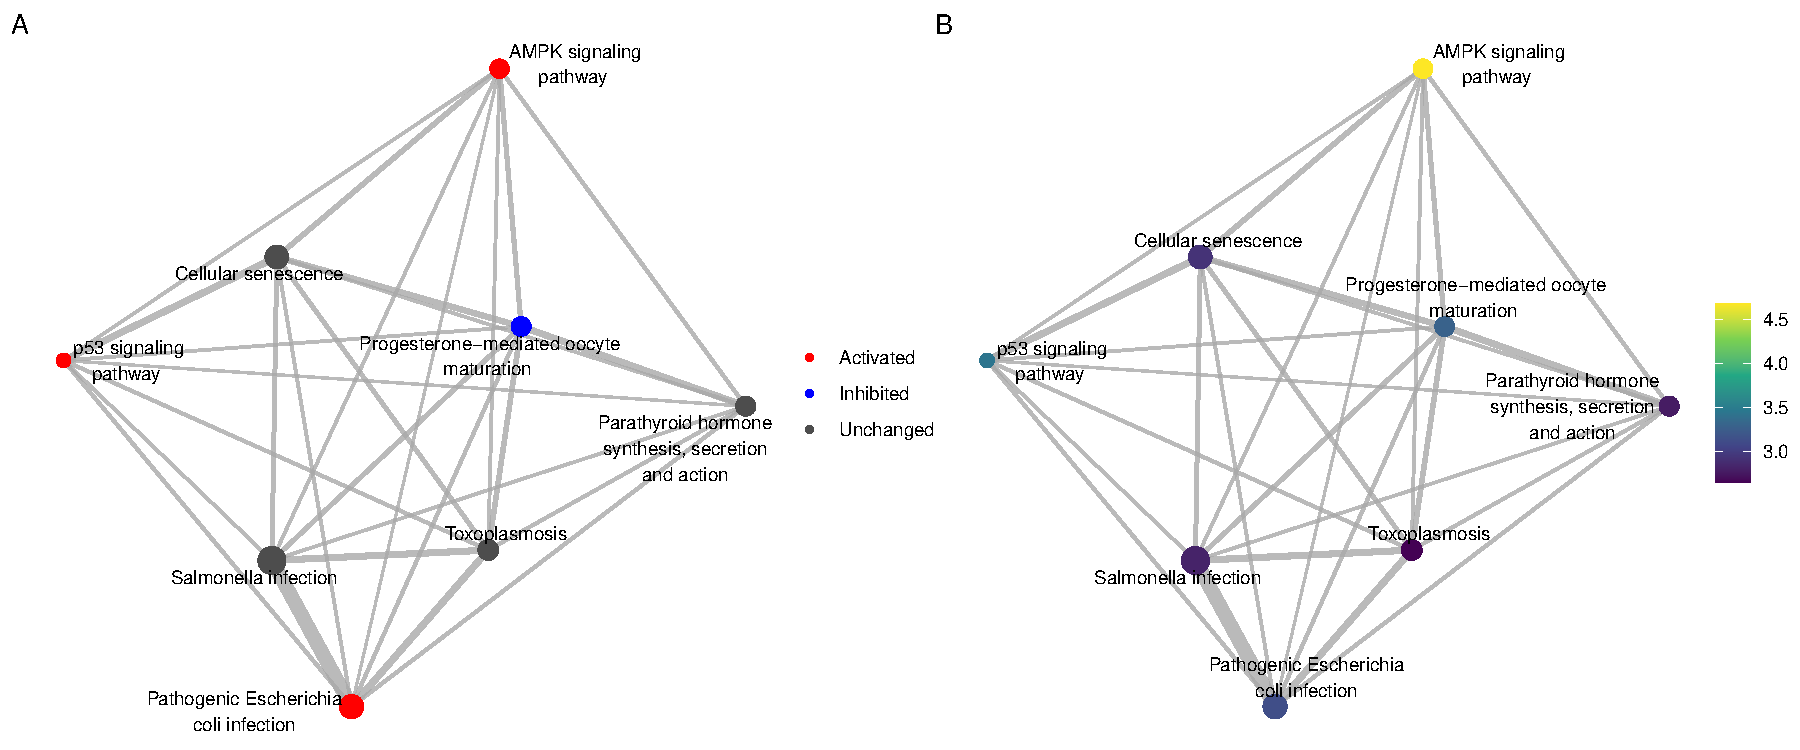
\includegraphics[width=1\linewidth]{sSNAPPY_paper_files/figure-latex/Figure1-1} 

}

\caption{Significantly perturbed KEGG pathways identified among post-chemotherapy samples using sSNAPPY, colored by (A) pathways’ predicted directions of changes and (B) pathways’ -log10(p-values). Pathways with a FDR < 0.05 in the moderated t-test were included.}\label{fig:Figure1}
\end{figure}

By examining the network structure, we can see that many of the highly connected pathways playing a central role in the network may be immune-related.
To summarise related pathways and further enable interpretation, we use community detection to group related pathways
Widely used in network analysis, community detection is a technique for identifying groups of nodes that are more densely connected than to any other nodes in the network\citep{Newman2004}.
sSNAPPY's \texttt{plot\_community()} function is a one-stop shop for applying a community detection algorithm of the user's choice to the network structure and annotating identified communities by the most common pathway category, denoting the main biological processes perturbed in that community.
Retrieved directly from the \href{https://www.genome.jp/kegg/pathway.html}{KEGG website}, we have curated the most recent categories for KEGG pathways and included this as part of sSNAPPY.
Annotation of KEGG pathway communities will be automatically completed by calling the in-built data object.
However, analyses involving other pathway databases will require user-provided pathway categories.
In the current dataset, the Louvain method was applied to the network of biological pathways and revealed two primary communities, where one was annotated to be endocrine system related and the other one was clearly related to infectious diseases and the immune system (Figure \ref{fig:Figure2}).

\begin{Shaded}
\begin{Highlighting}[]
\FunctionTok{set.seed}\NormalTok{(}\DecValTok{123}\NormalTok{)}
\FunctionTok{plot\_community}\NormalTok{(}
  \AttributeTok{normalisedScores =}\NormalTok{ sigPathway, }
  \AttributeTok{gsTopology =}\NormalTok{ gsTopology, }
  \AttributeTok{colorBy =} \StringTok{"status"}\NormalTok{, }
\NormalTok{) }\SpecialCharTok{+}
  \FunctionTok{scale\_colour\_manual}\NormalTok{(}\AttributeTok{values =} \FunctionTok{c}\NormalTok{(}\StringTok{"red"}\NormalTok{, }\StringTok{"blue"}\NormalTok{, }\StringTok{"grey30"}\NormalTok{)) }\SpecialCharTok{+}
  \FunctionTok{scale\_x\_continuous}\NormalTok{(}\AttributeTok{expand =} \FunctionTok{expansion}\NormalTok{(}\FloatTok{0.2}\NormalTok{)) }\SpecialCharTok{+}
  \FunctionTok{scale\_y\_continuous}\NormalTok{(}\AttributeTok{expand =} \FunctionTok{expansion}\NormalTok{(}\FloatTok{0.2}\NormalTok{)) }\SpecialCharTok{+}
  \FunctionTok{theme\_void}\NormalTok{()}
\end{Highlighting}
\end{Shaded}

\begin{figure}

{\centering 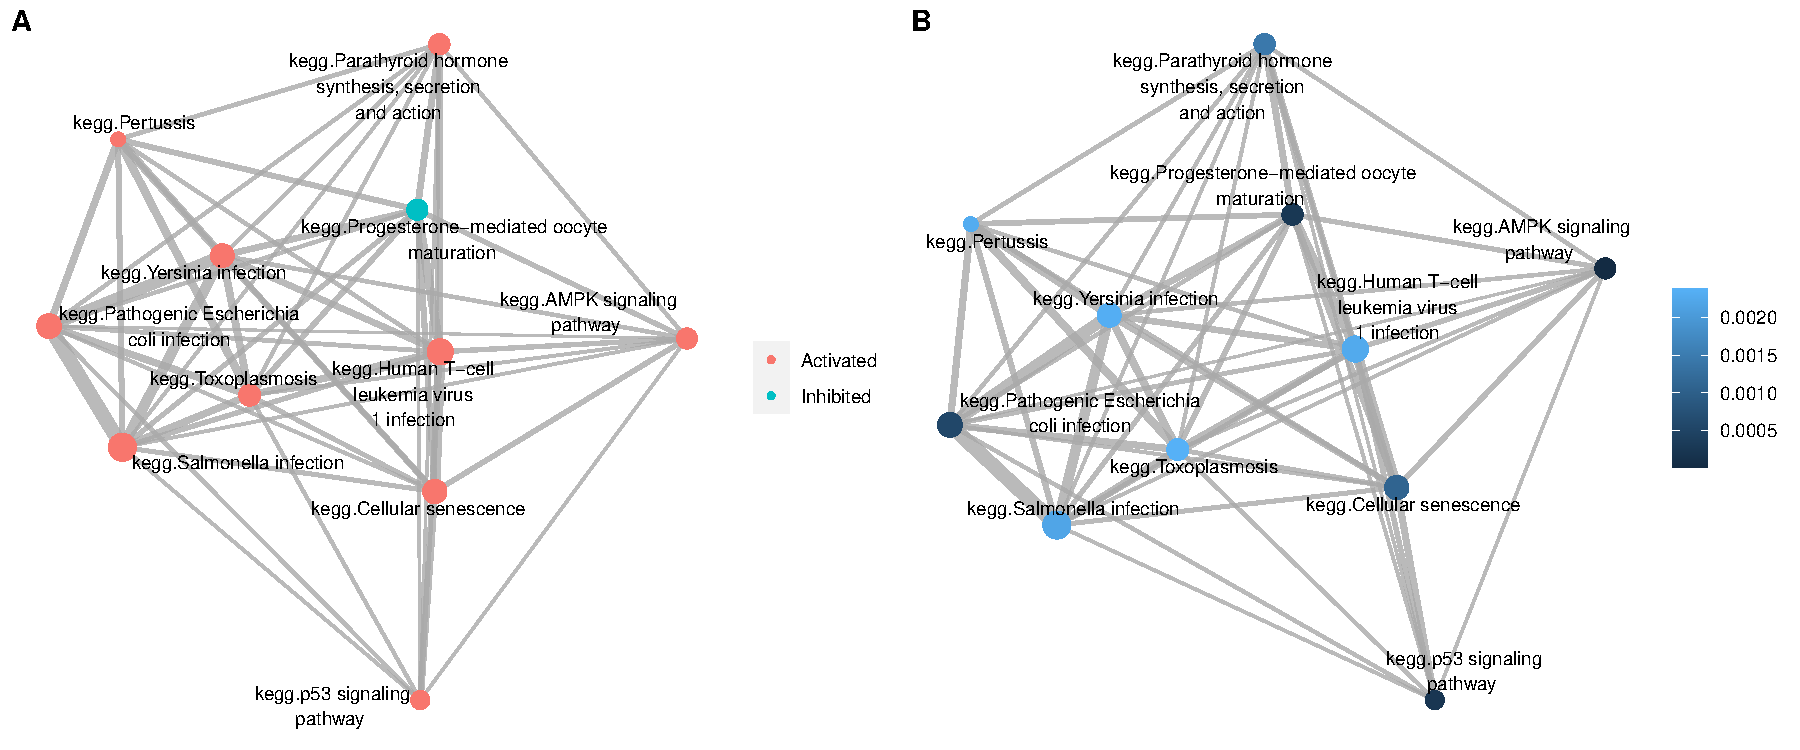
\includegraphics[width=0.8\linewidth]{sSNAPPY_paper_files/figure-latex/Figure2-1} 

}

\caption{Significantly perturbed KEGG pathways identified among post-chemotherapy samples using sSNAPPY, colored by (A) pathways’ predicted directions of changes and (B) pathways’ -log10(p-values). Pathways with a FDR < 0.05 in the moderated t-test were included.}\label{fig:Figure2}
\end{figure}

Inferred directly from the expression matrix, a key advantage of sSNAPPY is that it does not require the prior identification of differentially expressed genes, which is not always possible in clinical datasets.
However, knowing which genes are implicated in the perturbation of pathways, particularly those which influence multiple pathways, can provide valuable insights for hypotheses generation about underlying biological mechanisms.
Therefore, sSNAPPY presents another visualisation feature called \texttt{plot\_gs2gene}, which enables the inclusion of select genes from each pathway using network structures.
Users can provide a vector of fold-change estimates to visualise genes within pathways, showing their estimated change in expression.
As pathways often include hundreds of genes, we recommend to filter for genes most likely to be playing a significant role.
In this example dataset, we chose to only include genes within the top 500 when ranking by the magnitude of the mean log fold-change (Figure \ref{fig:Figure3}).

\begin{Shaded}
\begin{Highlighting}[]
\NormalTok{meanFC }\OtherTok{\textless{}{-}} \FunctionTok{rowMeans}\NormalTok{(weightedFC}\SpecialCharTok{$}\NormalTok{logFC) }\SpecialCharTok{/}\NormalTok{ weightedFC}\SpecialCharTok{$}\NormalTok{weight}
\NormalTok{top500 }\OtherTok{\textless{}{-}} \FunctionTok{rank}\NormalTok{(}\DecValTok{1}\SpecialCharTok{/}\FunctionTok{abs}\NormalTok{(meanFC)) }\SpecialCharTok{\textless{}=} \DecValTok{500}
\NormalTok{dirFC }\OtherTok{\textless{}{-}} \FunctionTok{ifelse}\NormalTok{(meanFC }\SpecialCharTok{\textgreater{}} \DecValTok{0}\NormalTok{, }\StringTok{"Up{-}Regulated"}\NormalTok{, }\StringTok{"Down{-}Regulated"}\NormalTok{)}
\end{Highlighting}
\end{Shaded}

Since KEGG pathway topologies were retrieved using EntrezIDs, a mapping object for IDs to gene names can also be provided.
However, users can provide a data.frame mapping Entrez IDs to their chosen identifiers through the mapRownameTo parameter.
A data.frame converting Entrez IDs to ensemble gene names has been made available as part of the package.

\begin{Shaded}
\begin{Highlighting}[]
\FunctionTok{load}\NormalTok{(}\FunctionTok{system.file}\NormalTok{(}\StringTok{"extdata"}\NormalTok{, }\StringTok{"entrez2name.rda"}\NormalTok{, }\AttributeTok{package =} \StringTok{"sSNAPPY"}\NormalTok{))}
\FunctionTok{head}\NormalTok{(entrez2name)}
\end{Highlighting}
\end{Shaded}

\begin{verbatim}
## # A tibble: 6 x 3
##   gene_id         mapTo   entrezid          
##   <chr>           <chr>   <chr>             
## 1 ENSG00000223972 DDX11L1 ENTREZID:84771    
## 2 ENSG00000223972 DDX11L1 ENTREZID:727856   
## 3 ENSG00000223972 DDX11L1 ENTREZID:100287102
## 4 ENSG00000223972 DDX11L1 ENTREZID:100287596
## 5 ENSG00000223972 DDX11L1 ENTREZID:102725121
## 6 ENSG00000227232 WASH7P  ENTREZID:653635
\end{verbatim}

\begin{Shaded}
\begin{Highlighting}[]
\FunctionTok{set.seed}\NormalTok{(}\DecValTok{123}\NormalTok{)}
\FunctionTok{plot\_gs2gene}\NormalTok{(}
  \AttributeTok{normalisedScores =}\NormalTok{ sigPathway, }
  \AttributeTok{gsTopology =}\NormalTok{ gsTopology, }
  \AttributeTok{colorGsBy =} \StringTok{"status"}\NormalTok{, }
  \AttributeTok{mapEntrezID =}\NormalTok{ entrez2name, }
  \AttributeTok{geneFC =}\NormalTok{ meanFC[top500], }
  \AttributeTok{edgeAlpha =} \FloatTok{0.3}\NormalTok{, }
  \AttributeTok{gsNameSize =} \DecValTok{4}\NormalTok{, }\AttributeTok{gsNodeSize =} \DecValTok{4}
\NormalTok{) }\SpecialCharTok{+}
  \FunctionTok{scale\_colour\_gradient2}\NormalTok{(}\AttributeTok{name =} \StringTok{"logFC"}\NormalTok{) }\SpecialCharTok{+}
  \FunctionTok{scale\_fill\_manual}\NormalTok{(}\AttributeTok{values =} \FunctionTok{c}\NormalTok{(}\StringTok{"red"}\NormalTok{, }\StringTok{"blue"}\NormalTok{, }\StringTok{"grey50"}\NormalTok{)) }\SpecialCharTok{+}
  \FunctionTok{theme\_void}\NormalTok{()}
\end{Highlighting}
\end{Shaded}

\begin{figure}

{\centering 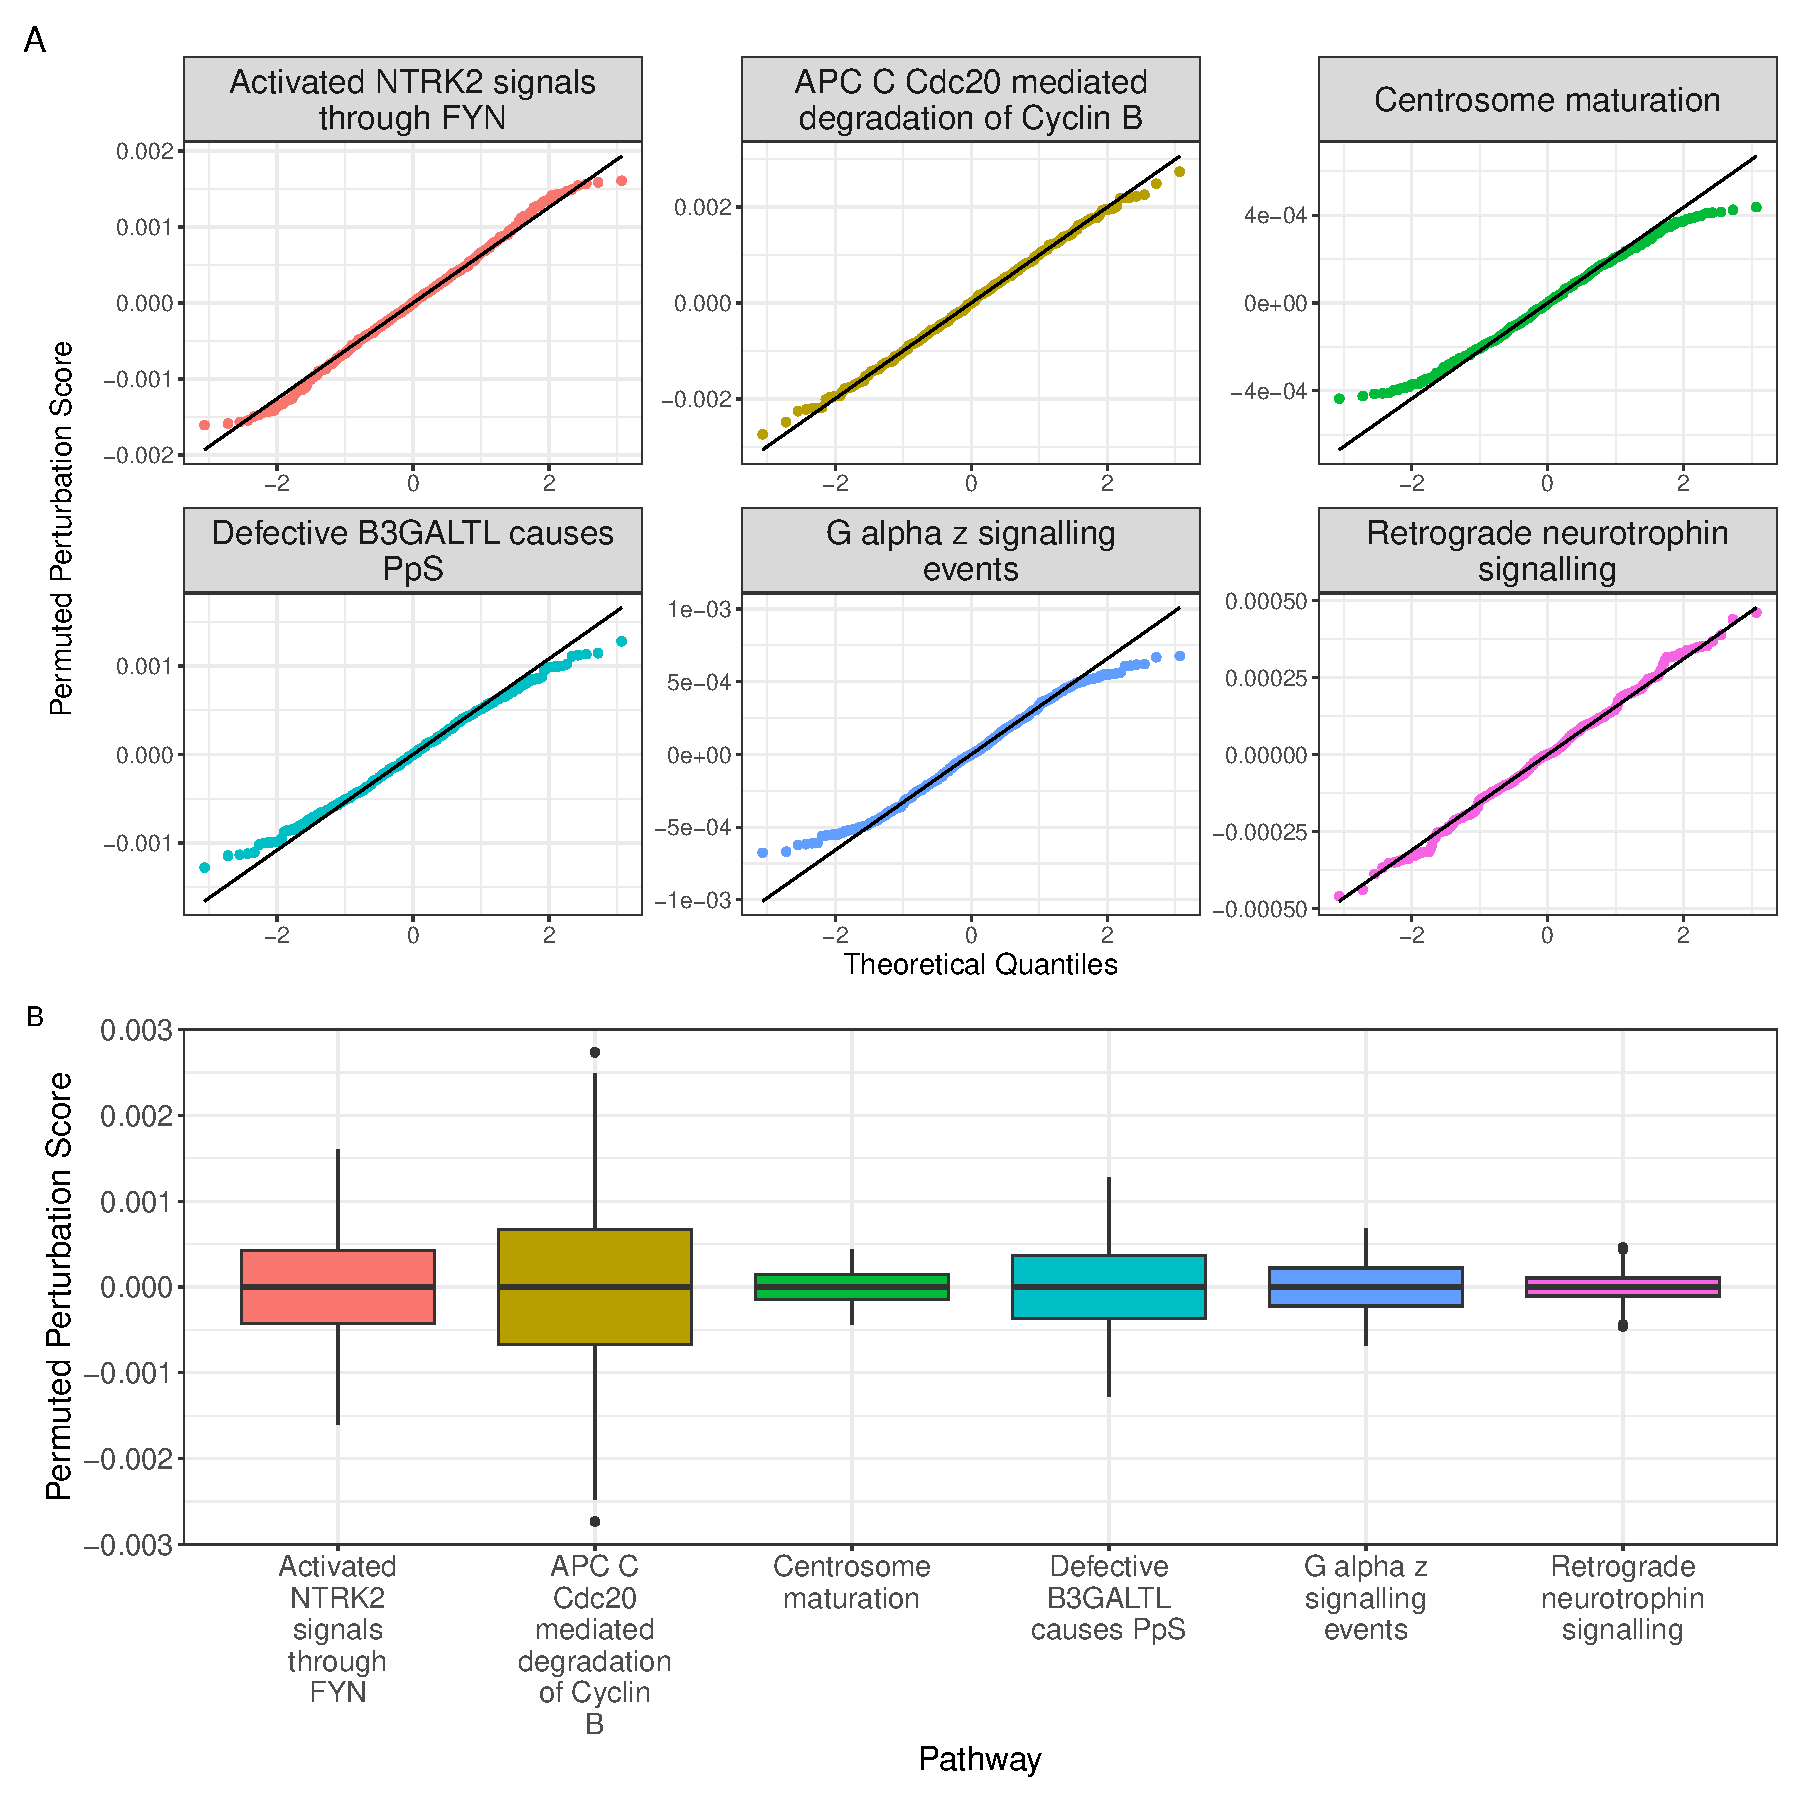
\includegraphics[width=0.8\linewidth]{sSNAPPY_paper_files/figure-latex/Figure3-1} 

}

\caption{Significantly perturbed KEGG pathways identified among post-chemotherapy samples using sSNAPPY, annotated by community structure identified with the Louvain algorithm.2 communities were formed, both of which were annotated by the pathway category that the majority of the pathways belong to. }\label{fig:Figure3}
\end{figure}

\hypertarget{identify-hub-genes-contributing-to-pathway-perturbation}{%
\subsection{Identify hub genes contributing to pathway perturbation}\label{identify-hub-genes-contributing-to-pathway-perturbation}}

If we would like to further investigate a specific pathway and elucidate the key genes that contributed to its perturbation, such as the activation of the ``p53 signalling pathway,'' we can employ a heatmap to display the gene-level perturbation scores of all the genes within the pathway and annotate each column (ie. each sample) by the direction of pathway perturbation in that sample or any other sample metadata using the plot\_gene\_contribution function (Figure \ref{fig:Figure4}).

\begin{Shaded}
\begin{Highlighting}[]
\FunctionTok{plot\_gene\_contribution}\NormalTok{(}
  \AttributeTok{genePertScore =}\NormalTok{ genePertScore, }
  \AttributeTok{gsToPlot =} \StringTok{"p53 signaling pathway"}\NormalTok{, }
  \AttributeTok{metadata =}\NormalTok{ dplyr}\SpecialCharTok{::}\FunctionTok{filter}\NormalTok{(sample\_meta, treatment }\SpecialCharTok{==} \StringTok{"post{-}NACT"}\NormalTok{) }\SpecialCharTok{\%\textgreater{}\%}
\NormalTok{    dplyr}\SpecialCharTok{::}\FunctionTok{select}\NormalTok{(}\AttributeTok{sample =}\NormalTok{ patient\_id, Stage), }
  \AttributeTok{annotation\_attribute =} \FunctionTok{c}\NormalTok{(}\StringTok{"pathwayPertScore"}\NormalTok{, }\StringTok{"Stage"}\NormalTok{), }
  \AttributeTok{pathwayPertScore =}\NormalTok{ ssPertScore, }
  \AttributeTok{mapEntrezID =}\NormalTok{ entrez2name}
\NormalTok{)}
\end{Highlighting}
\end{Shaded}

\begin{figure}

{\centering 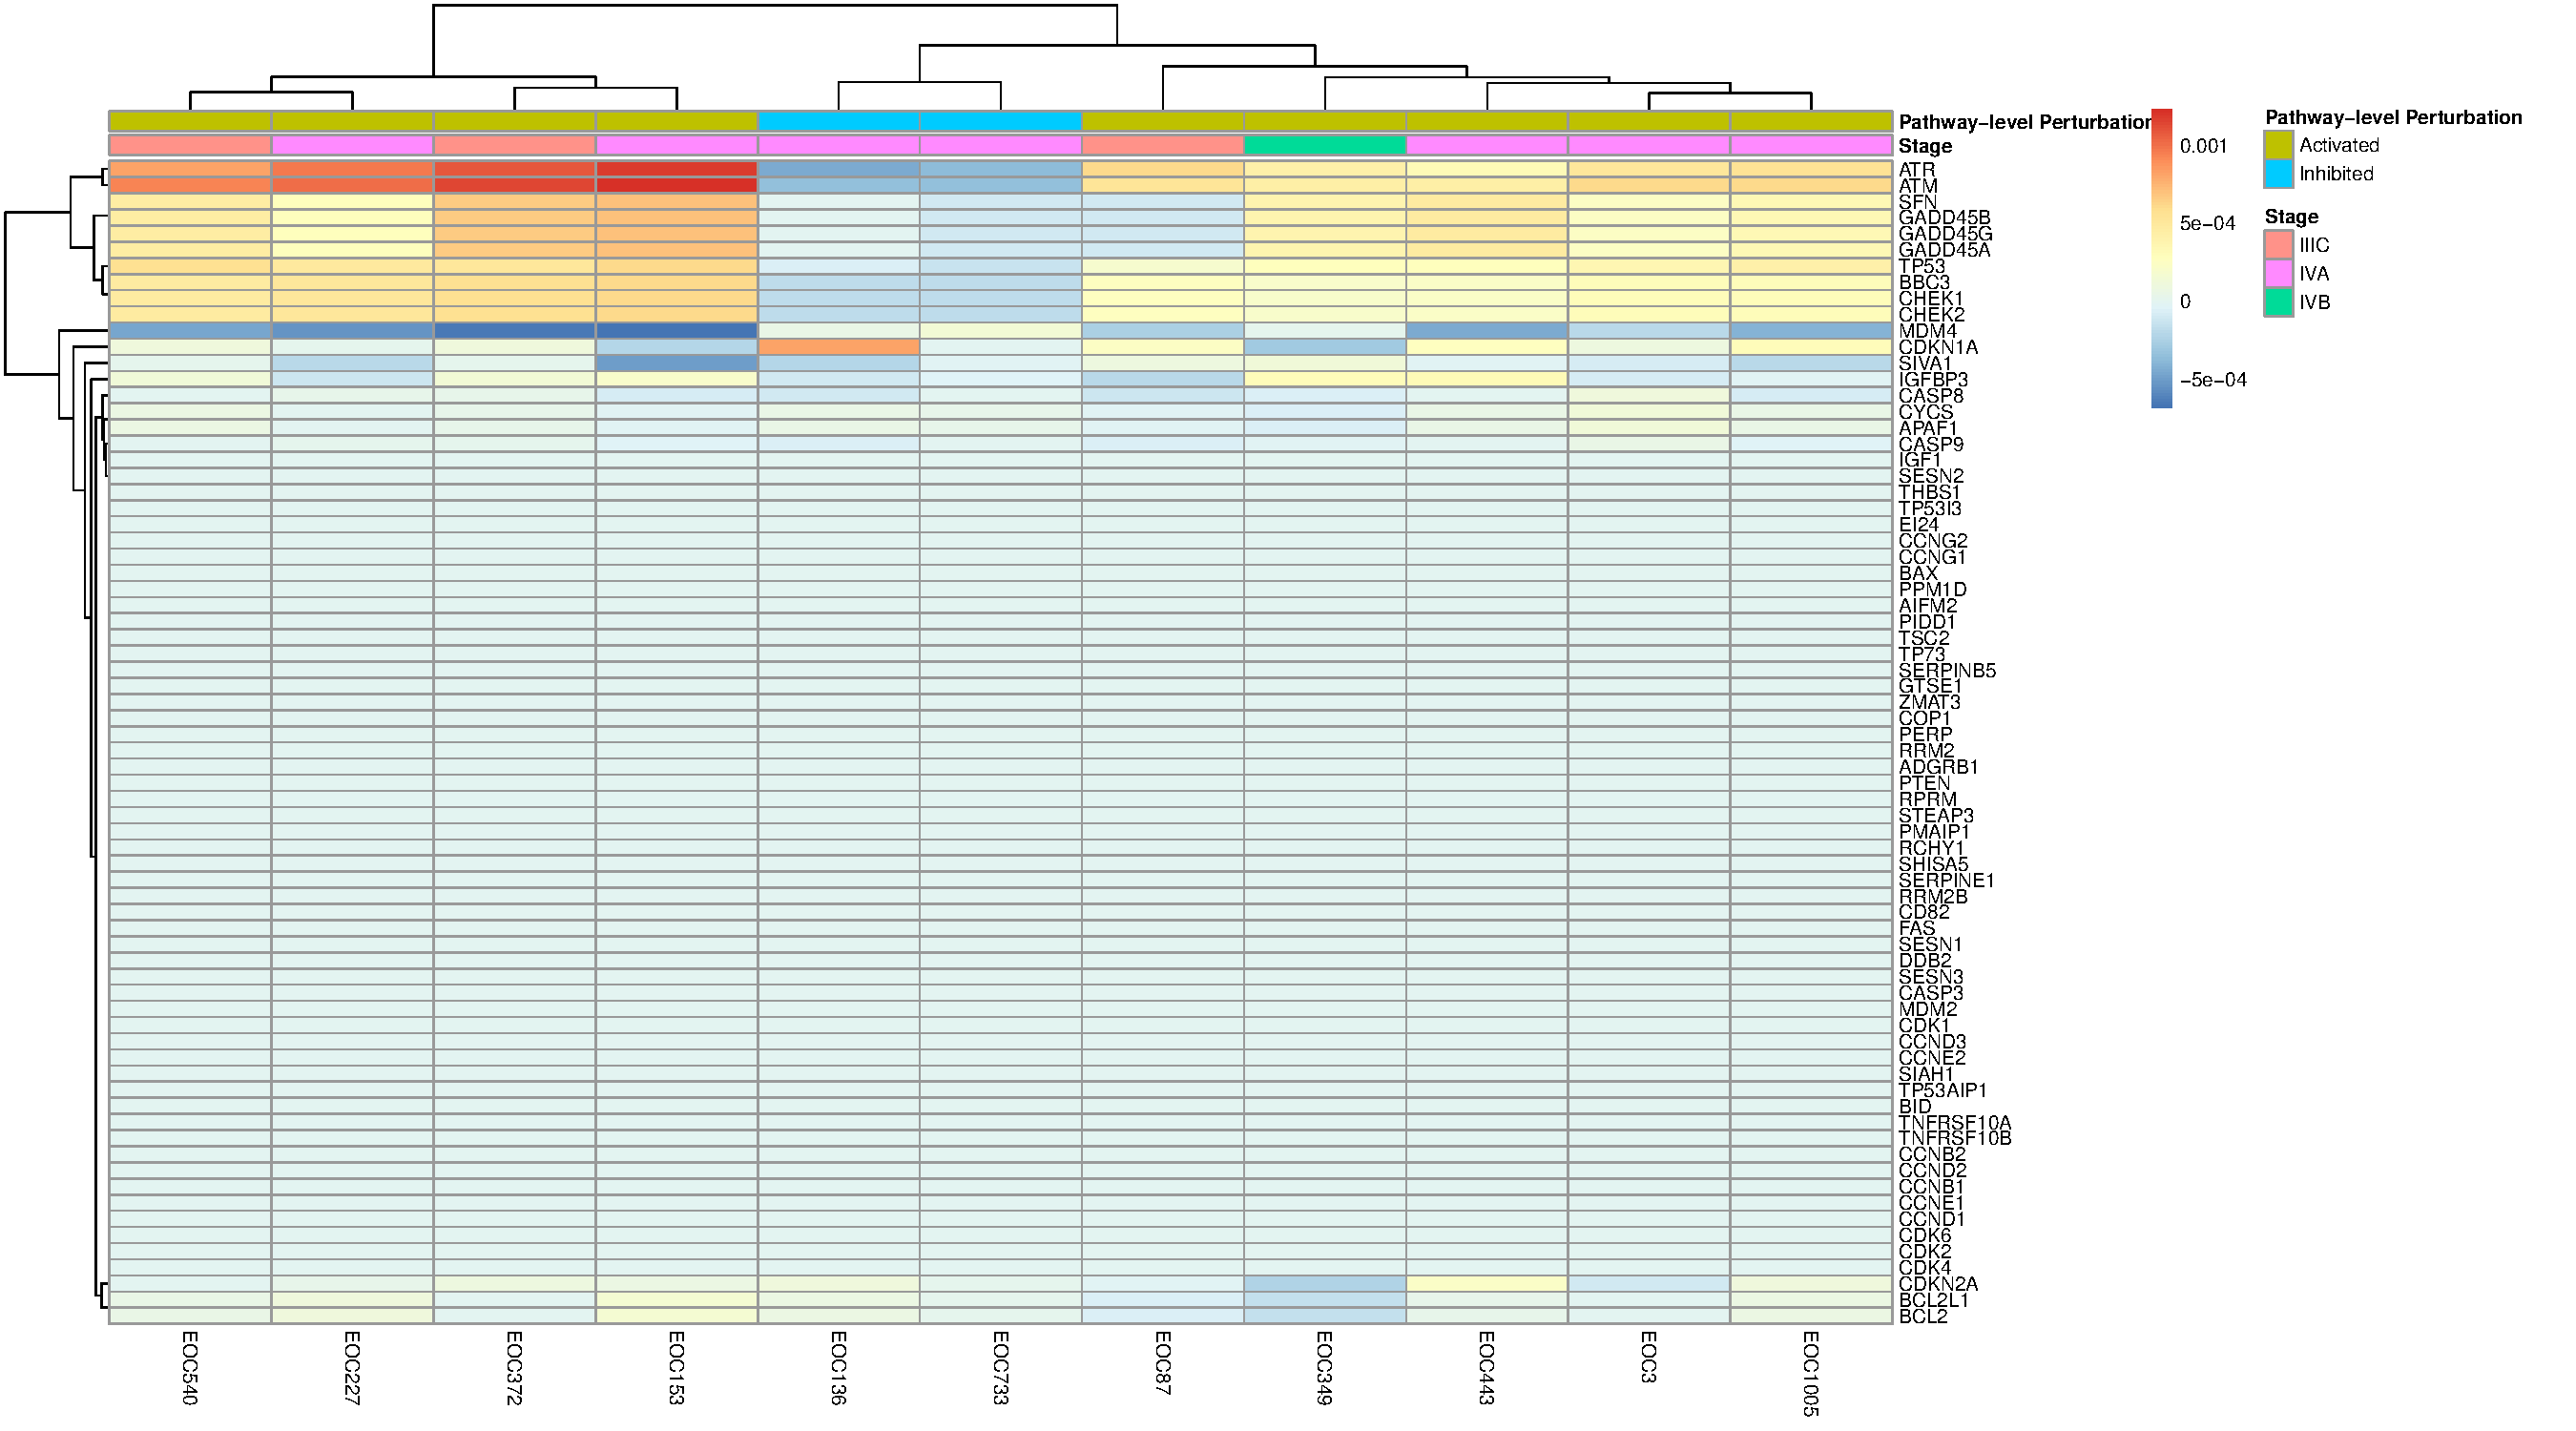
\includegraphics[width=1\linewidth]{sSNAPPY_paper_files/figure-latex/Figure4-1} 

}

\caption{Gene-level perturbation scores of all genes included in the "p53 signalling pathway" pathway in each sample where columns of samples were annotated by pathway-level perturbation and the stages of cancers. Genes ATR and ATM were the key driver of the activation of p53 signalling pathway. }\label{fig:Figure4}
\end{figure}

From this heatmap we can easily identify that the hub genes making the biggest contribution to the activation of p53 signalling pathway upon chemotherapy were gene ART and gene ATM. The Ataxia-telangiectasia mutated (ATM) gene is a well-established oncosuppressor\citep{Moslemi2021}, mutation of which has been observed in many types of cancers\citep{Choi2016}. Also involved in DNA damage repair, the Ataxia telangiectasia and RAD3-related protein kinase (ATR) gene has been shown to be a promising therapeutic target for HGSOC\citep{Li2022}.

\hypertarget{discussion}{%
\section{Discussion}\label{discussion}}

In conclusion, the paper showcased an R/Bioconductor package that offers a novel single-sample pathway perturbation testing approach. sSNAPPY utilizes pathway topology information to compute perturbation scores that predict pathways' potential directions of changes in individual samples. This approach addresses the limitations of current strategies that fail to account for gene-gene interactions encoded by pathway topologies or predict the directionality of pathway activities. By applying sSNAPPY to a public scRNA-seq data collected before and after HGSOC patients were subjected to chemotherapy, we demonstrated its ability to detect significant pathway perturbations of various interesting biological processes beyond what were shown in the original studies. Overall, sSNAPPY presents a promising strategy for single sample-based pathway analysis in RNA-seq data.

\hypertarget{data-availability}{%
\section{Data availability}\label{data-availability}}

The dataset analysed in this manuscript are stored in the data directory of this GitHub repository.

\hypertarget{software-availability}{%
\section{Software availability}\label{software-availability}}

\begin{itemize}
\item
  Software available from: \url{https://bioconductor.org/packages/release/bioc/html/sSNAPPY.html}
\item
  Source code available from: \url{https://github.com/Wenjun-Liu/sSNAPPY}
\item
  Archived source code at time of publication: {[}DOI (found on right hand side of a Zenodo record){]}
\item
  License: \href{https://opensource.org/license/mit/}{MIT}
\end{itemize}

\hypertarget{competing-interests}{%
\section{Competing interests}\label{competing-interests}}

No competing interests were disclosed

\hypertarget{grant-information}{%
\section{Grant information}\label{grant-information}}

Any grants that supported the work must be listed here, including the grant number.

\renewcommand\refname{Acknowledgements}
{\small\bibliography{sample.bib}}

\end{document}
